\section{Results}
\label{sec:results}

\ifnum\lgwHasResults=0
\textit{No inference run has been analysed. Every table and number below is a
generated placeholder; see the note on the title page.}
\else
Run: \lgwModel, $n_{\text{anom}} = \lgwNAnom$, $d = \lgwDim$. Source:
\lgwSource. \lgwNote
\fi

At the pre-registered operating point, \texttt{loss\_L0} alarmed on 36.6\% of anomalous clips against a held-out clip-level false-alarm rate of 14.0\% (lift +0.226); \texttt{loss\_L1} alarmed on 70.8\% of anomalous clips against a held-out clip-level false-alarm rate of 10.0\% (lift +0.608).

Both baselines detect anomalies above chance, so the comparison against them is meaningful.

The strongest probe by RMTA is \texttt{probe\_B}, whose worst-case gain against either baseline is -2.05 frames; against \texttt{loss\_L0} its RMTA gain is +1.88 frames (95\% CI [+1.48, +2.26], Holm-adjusted $p=0.003$).

No probe satisfies the frozen Early Warner criterion (a median gain of at least one frame against both baselines at Holm-adjusted $p<0.01$).

Re-deriving thresholds so the clip-level false-alarm rate is 5\% rather than matching the per-frame rate does not change the picture: the Early Warner set becomes empty.


\begin{table}[t]
\centering
\small
\begin{tabular}{lrrrrrr}
\toprule
Monitor & median $\Delta t$ & RMTA & 95\% CI & detect. & clip FPR & lift \\
\midrule
$\mathcal{L}_0$ (V-JEPA 2 own loss) & 14.0 & 10.37 & [10.01, 10.70] & 0.366 & 0.140 & +0.226 \\
$\mathcal{L}_1$ (ridge, info-matched) & 4.0 & 6.45 & [6.08, 6.80] & 0.708 & 0.100 & +0.608 \\
\midrule
$\mathrm{A}$: curvature & 14.0 & 9.40 & [9.02, 9.75] & 0.424 & 0.120 & +0.304 \\
$\mathrm{B}$: repr.\ distance & 14.0 & 8.49 & [8.09, 8.89] & 0.490 & 0.130 & +0.360 \\
$\mathrm{C}$: covariance shift & 14.0 & 13.05 & [12.86, 13.23] & 0.179 & 0.040 & +0.139 \\
\bottomrule
\end{tabular}

\caption{Time-to-alarm per monitor at the pre-registered operating point
(per-frame false-alarm rate matched at $1\%$). \emph{Lift} is detection rate
minus held-out clip-level false-alarm rate; $\dagger$ marks a monitor firing at
chance. RMTA is the restricted mean time-to-alarm in frames, lower being
earlier, with a percentile bootstrap interval.}
\label{tab:tta}
\end{table}

\begin{table}[t]
\centering
\small
\begin{tabular}{lrrrrr}
\toprule
Comparison & median gain & RMTA gain & 95\% CI & $p$ (Holm) & $p$ (Holm, RMTA) \\
\midrule
\texttt{probe\_A\_vs\_loss\_L0} & +0.0 & +0.98 & [+0.70, +1.26] & $<10^{-4}$ & 0.003 \\
\texttt{probe\_A\_vs\_loss\_L1} & -10.0 & -2.95 & [-3.23, -2.68] & 1 & 1 \\
\texttt{probe\_B\_vs\_loss\_L0} & +0.0 & +1.88 & [+1.48, +2.26] & $<10^{-4}$ & 0.003 \\
\texttt{probe\_B\_vs\_loss\_L1} & -10.0 & -2.05 & [-2.33, -1.78] & 1 & 1 \\
\texttt{probe\_C\_vs\_loss\_L0} & +0.0 & -2.68 & [-3.05, -2.32] & 1 & 1 \\
\texttt{probe\_C\_vs\_loss\_L1} & -10.0 & -6.60 & [-7.00, -6.23] & 1 & 1 \\
\bottomrule
\end{tabular}

\caption{Paired probe-versus-baseline comparisons. Positive gain means the
probe alarms earlier. $p$ values are Holm-adjusted across all six comparisons;
the RMTA column uses the paired cluster bootstrap. A probe is an Early Warner
only if it achieves a median gain of at least one frame against \emph{both}
baselines at adjusted $p<0.01$.}
\label{tab:cmp}
\end{table}

\begin{figure}[t]
\centering
\IfFileExists{generated/fig_survival.png}{%
  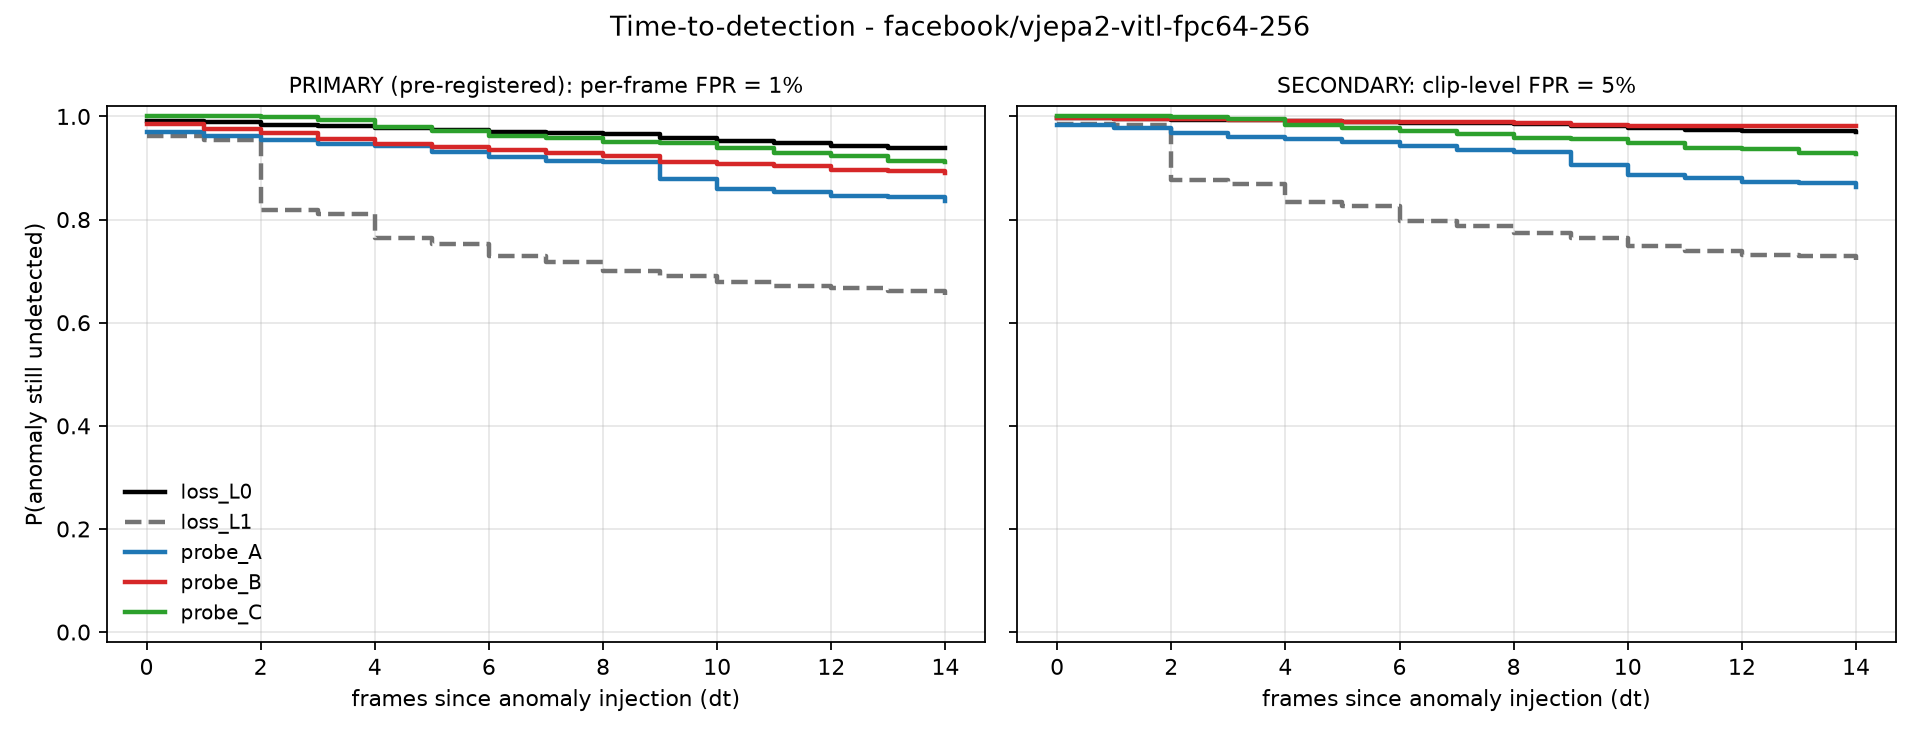
\includegraphics[width=\linewidth]{generated/fig_survival.png}}{%
  \fbox{\parbox{0.8\linewidth}{\centering\vspace{18pt}\textsc{pending}\\[2pt]
  \footnotesize survival curves are produced by the analysis run\vspace{18pt}}}}
\caption{Kaplan--Meier curves for time-to-detection under both threshold
regimes: the probability that an anomaly remains undetected $\dt$ frames after
injection. A monitor that warns earlier drops sooner. Curves that stay flat
near $1$ indicate a monitor that mostly fails to fire inside the window, which
is the regime in which the median is uninformative.}
\label{fig:survival}
\end{figure}

\begin{table}[t]
\centering
\small
\begin{tabular}{lrrrr}
\toprule
Monitor & gravity inv. & friction & occlusion & frame drop \\
\midrule
$\mathcal{L}_0$ (V-JEPA 2 own loss) & 12.59 & 13.08 & 13.59 & 2.23 \\
$\mathcal{L}_1$ (ridge, info-matched) & 10.56 & 12.74 & 1.50 & 0.98 \\
\midrule
$\mathrm{A}$: curvature & 13.62 & 13.56 & 8.95 & 1.45 \\
$\mathrm{B}$: repr.\ distance & 13.14 & 12.86 & 4.88 & 3.10 \\
$\mathrm{C}$: covariance shift & 13.43 & 13.62 & 12.72 & 12.42 \\
\bottomrule
\end{tabular}

\caption{RMTA by anomaly condition (frames; lower is earlier). Conditions
differ in disturbance magnitude, so these are not comparable across columns ---
they show \emph{where} any effect is concentrated, not which anomaly is
``easier''.}
\label{tab:cond}
\end{table}

\begin{table}[t]
\centering
\small
\begin{tabular}{lrrrr}
\toprule
Monitor & median $\Delta t$ & RMTA & detect. & clip FPR \\
\midrule
$\mathcal{L}_0$ (V-JEPA 2 own loss) & 14.0 & 10.67 & 0.330 & 0.100 \\
$\mathcal{L}_1$ (ridge, info-matched) & 7.0 & 7.21 & 0.621 & 0.020 \\
\midrule
$\mathrm{A}$: curvature & 14.0 & 10.09 & 0.357 & 0.080 \\
$\mathrm{B}$: repr.\ distance & 14.0 & 9.44 & 0.408 & 0.040 \\
$\mathrm{C}$: covariance shift & 14.0 & 12.94 & 0.194 & 0.050 \\
\bottomrule
\end{tabular}

\caption{The secondary operating point: thresholds re-derived so the
clip-level false-alarm rate on calibration controls is $5\%$. Registered before
any inference run and reported unconditionally.}
\label{tab:secondary}
\end{table}

\subsection{Reading these tables honestly}

Three questions should be asked of Table~\ref{tab:tta} before
Table~\ref{tab:cmp} is read at all.

\emph{Do the baselines detect anything?} If a baseline's lift is near zero it
fires at chance, and every comparison against it in Table~\ref{tab:cmp} is
uninformative about the hypothesis regardless of its $p$ value. The
$\dagger$ marker and the \textsc{vacuous} flag exist for this case.

\emph{Is the median degenerate?} If detection rates are below $50\%$, the median
$\dt$ column will read identically for every monitor and the median-gain column
of Table~\ref{tab:cmp} will be all zeros. That is an artefact of censoring, not
evidence of equality; the RMTA columns are the ones carrying information.

\emph{Does the conclusion survive the second operating point?} A result that
appears at a $1\%$ per-frame threshold and vanishes at a $5\%$ clip-level
threshold is an operating-point artefact, not a property of the
representation.

\subsection{Gate}

The frozen decision rule returns \textbf{\lgwVerdict}. Early warners under the
registered primary: \lgwEarlyWarners. Under the censoring-robust secondary:
\lgwRmtaWarners. Median degenerate: \lgwMedianDegenerate. Baselines firing at
chance: \lgwBaselinesAtChance. Verdict vacuous: \lgwVacuous.
